\section{Generated non-manual breadth monitor}
\label{app:nonmanual-breadth-auto}

This section is generated automatically by the overnight controller.  It is
included to remove ambiguity between clean paper-level claims and broader
stress tests.  A row marked mixed is not promoted to a main-text claim; it
identifies an environment-age setting that requires confirmation or a design
change.

\paragraph{Generation status.} Overnight sequence completed. Last update: 2026-07-17T02:57:48.

\paragraph{Random patch-set breadth wave.}
This generated block reports 13/21 environment-age rows passing the
registered non-manual gate. Mixed rows are treated as stress-test limits or
confirmation targets, not as headline wins.

\begin{figure}[!tbp]
\centering
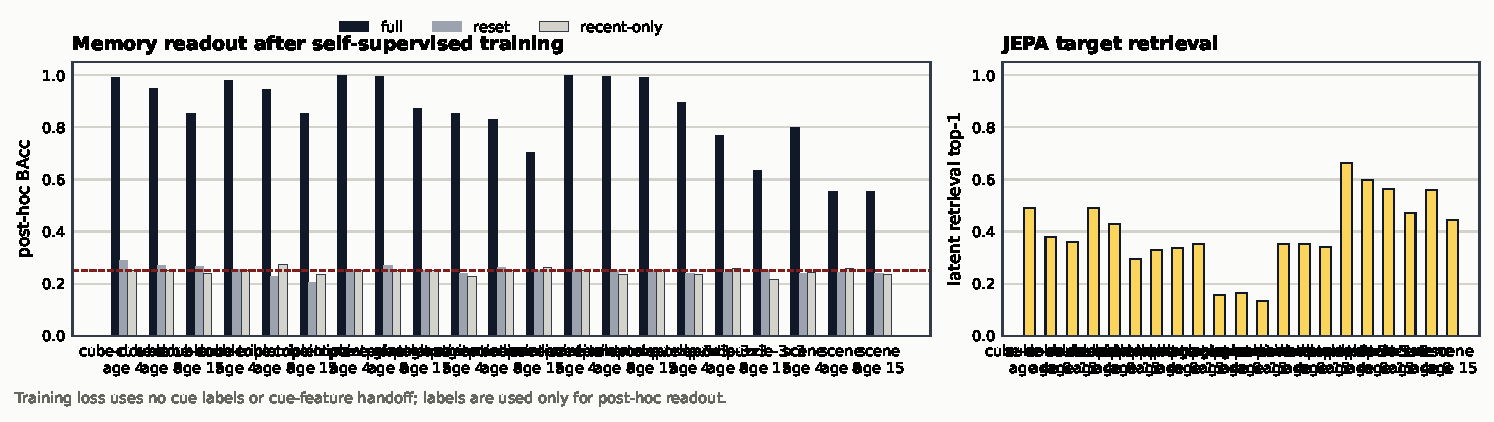
\includegraphics[width=\linewidth]{figures/fig_b_nonmanual_breadth_auto.pdf}
\caption{Generated non-manual breadth plot for Random patch-set breadth wave.}
\end{figure}

\begin{table}[!tbp]
\centering
\scriptsize
\setlength{\tabcolsep}{3.5pt}
\renewcommand{\arraystretch}{1.05}
\caption{Generated non-manual breadth table for Random patch-set breadth wave.}
\begin{tabular}{lccccccl}
\toprule
Deck & Age & Seeds & Pass & Full & Reset & Recent & Status\\
\midrule
cube-double-play-v0 & 4 & 3 & 3/3 & 0.991 & 0.289 & 0.250 & \textsc{pass}\\
cube-double-play-v0 & 8 & 3 & 2/3 & 0.949 & 0.270 & 0.249 & \textsc{mixed}\\
cube-double-play-v0 & 15 & 3 & 3/3 & 0.854 & 0.266 & 0.238 & \textsc{pass}\\
cube-triple-play-v0 & 4 & 3 & 3/3 & 0.981 & 0.255 & 0.251 & \textsc{pass}\\
cube-triple-play-v0 & 8 & 3 & 3/3 & 0.947 & 0.228 & 0.275 & \textsc{pass}\\
cube-triple-play-v0 & 15 & 3 & 3/3 & 0.852 & 0.206 & 0.237 & \textsc{pass}\\
pointmaze-giant-navigate-v0 & 4 & 3 & 3/3 & 1.000 & 0.250 & 0.250 & \textsc{pass}\\
pointmaze-giant-navigate-v0 & 8 & 3 & 3/3 & 0.993 & 0.271 & 0.250 & \textsc{pass}\\
pointmaze-giant-navigate-v0 & 15 & 3 & 3/3 & 0.874 & 0.250 & 0.250 & \textsc{pass}\\
pointmaze-medium-navigate-v0 & 4 & 3 & 3/3 & 0.853 & 0.240 & 0.228 & \textsc{pass}\\
pointmaze-medium-navigate-v0 & 8 & 3 & 2/3 & 0.830 & 0.262 & 0.251 & \textsc{mixed}\\
pointmaze-medium-navigate-v0 & 15 & 3 & 1/3 & 0.702 & 0.249 & 0.263 & \textsc{mixed}\\
pointmaze-teleport-navigate-v0 & 4 & 3 & 3/3 & 1.000 & 0.250 & 0.249 & \textsc{pass}\\
pointmaze-teleport-navigate-v0 & 8 & 3 & 3/3 & 0.996 & 0.250 & 0.235 & \textsc{pass}\\
pointmaze-teleport-navigate-v0 & 15 & 3 & 3/3 & 0.993 & 0.250 & 0.250 & \textsc{pass}\\
puzzle-3x3-play-v0 & 4 & 3 & 3/3 & 0.896 & 0.238 & 0.234 & \textsc{pass}\\
puzzle-3x3-play-v0 & 8 & 3 & 1/3 & 0.770 & 0.242 & 0.259 & \textsc{mixed}\\
puzzle-3x3-play-v0 & 15 & 3 & 1/3 & 0.636 & 0.250 & 0.218 & \textsc{mixed}\\
scene-play-v0 & 4 & 3 & 2/3 & 0.799 & 0.238 & 0.243 & \textsc{mixed}\\
scene-play-v0 & 8 & 3 & 0/3 & 0.553 & 0.243 & 0.257 & \textsc{mixed}\\
scene-play-v0 & 15 & 3 & 0/3 & 0.552 & 0.239 & 0.235 & \textsc{mixed}\\
\bottomrule
\end{tabular}
\end{table}

\paragraph{Large-bank confirmation.}
This generated block reports 8/12 environment-age rows passing the
registered non-manual gate. Mixed rows are treated as stress-test limits or
confirmation targets, not as headline wins.

\begin{figure}[!tbp]
\centering
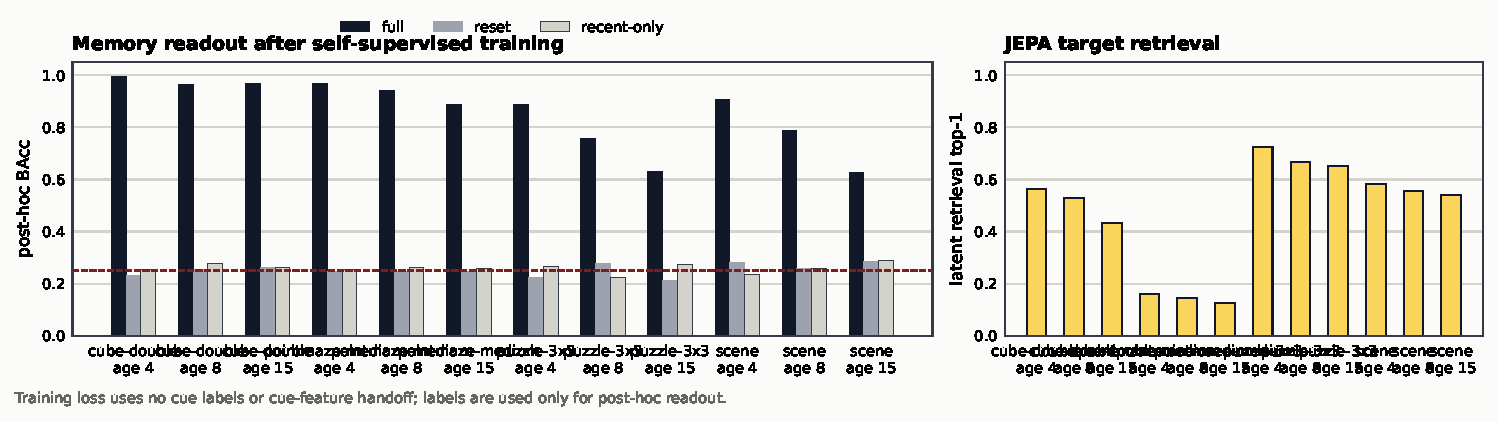
\includegraphics[width=\linewidth]{figures/fig_b_nonmanual_breadth_confirm_auto.pdf}
\caption{Generated non-manual breadth plot for Large-bank confirmation.}
\end{figure}

\begin{table}[!tbp]
\centering
\scriptsize
\setlength{\tabcolsep}{3.5pt}
\renewcommand{\arraystretch}{1.05}
\caption{Generated non-manual breadth table for Large-bank confirmation.}
\begin{tabular}{lccccccl}
\toprule
Deck & Age & Seeds & Pass & Full & Reset & Recent & Status\\
\midrule
cube-double-play-v0 & 4 & 3 & 3/3 & 0.995 & 0.233 & 0.255 & \textsc{pass}\\
cube-double-play-v0 & 8 & 3 & 3/3 & 0.964 & 0.253 & 0.277 & \textsc{pass}\\
cube-double-play-v0 & 15 & 3 & 3/3 & 0.969 & 0.264 & 0.263 & \textsc{pass}\\
pointmaze-medium-navigate-v0 & 4 & 3 & 3/3 & 0.968 & 0.248 & 0.255 & \textsc{pass}\\
pointmaze-medium-navigate-v0 & 8 & 3 & 3/3 & 0.941 & 0.249 & 0.263 & \textsc{pass}\\
pointmaze-medium-navigate-v0 & 15 & 3 & 3/3 & 0.888 & 0.246 & 0.260 & \textsc{pass}\\
puzzle-3x3-play-v0 & 4 & 3 & 3/3 & 0.888 & 0.225 & 0.265 & \textsc{pass}\\
puzzle-3x3-play-v0 & 8 & 3 & 1/3 & 0.757 & 0.277 & 0.225 & \textsc{mixed}\\
puzzle-3x3-play-v0 & 15 & 3 & 0/3 & 0.632 & 0.212 & 0.272 & \textsc{mixed}\\
scene-play-v0 & 4 & 3 & 3/3 & 0.906 & 0.282 & 0.237 & \textsc{pass}\\
scene-play-v0 & 8 & 3 & 1/3 & 0.787 & 0.260 & 0.257 & \textsc{mixed}\\
scene-play-v0 & 15 & 3 & 0/3 & 0.626 & 0.286 & 0.288 & \textsc{mixed}\\
\bottomrule
\end{tabular}
\end{table}

\paragraph{antmaze-large-navigate-v0.}
This generated block reports 3/3 environment-age rows passing the
registered non-manual gate. Mixed rows are treated as stress-test limits or
confirmation targets, not as headline wins.

\begin{figure}[!tbp]
\centering
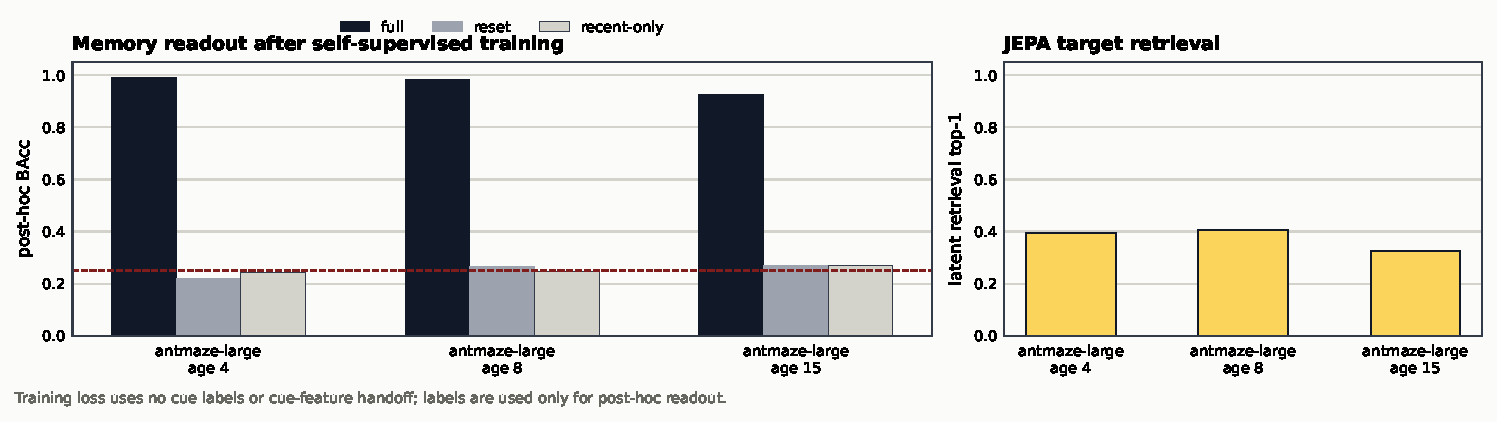
\includegraphics[width=\linewidth]{figures/fig_b_nonmanual_extra_antmaze_large_navigate_v0.pdf}
\caption{Generated non-manual breadth plot for antmaze-large-navigate-v0.}
\end{figure}

\begin{table}[!tbp]
\centering
\scriptsize
\setlength{\tabcolsep}{3.5pt}
\renewcommand{\arraystretch}{1.05}
\caption{Generated non-manual breadth table for antmaze-large-navigate-v0.}
\begin{tabular}{lccccccl}
\toprule
Deck & Age & Seeds & Pass & Full & Reset & Recent & Status\\
\midrule
antmaze-large-navigate-v0 & 4 & 3 & 3/3 & 0.992 & 0.220 & 0.243 & \textsc{pass}\\
antmaze-large-navigate-v0 & 8 & 3 & 3/3 & 0.985 & 0.264 & 0.245 & \textsc{pass}\\
antmaze-large-navigate-v0 & 15 & 3 & 3/3 & 0.925 & 0.268 & 0.271 & \textsc{pass}\\
\bottomrule
\end{tabular}
\end{table}

\paragraph{antmaze-giant-navigate-v0.}
This generated block reports 3/3 environment-age rows passing the
registered non-manual gate. Mixed rows are treated as stress-test limits or
confirmation targets, not as headline wins.

\begin{figure}[!tbp]
\centering
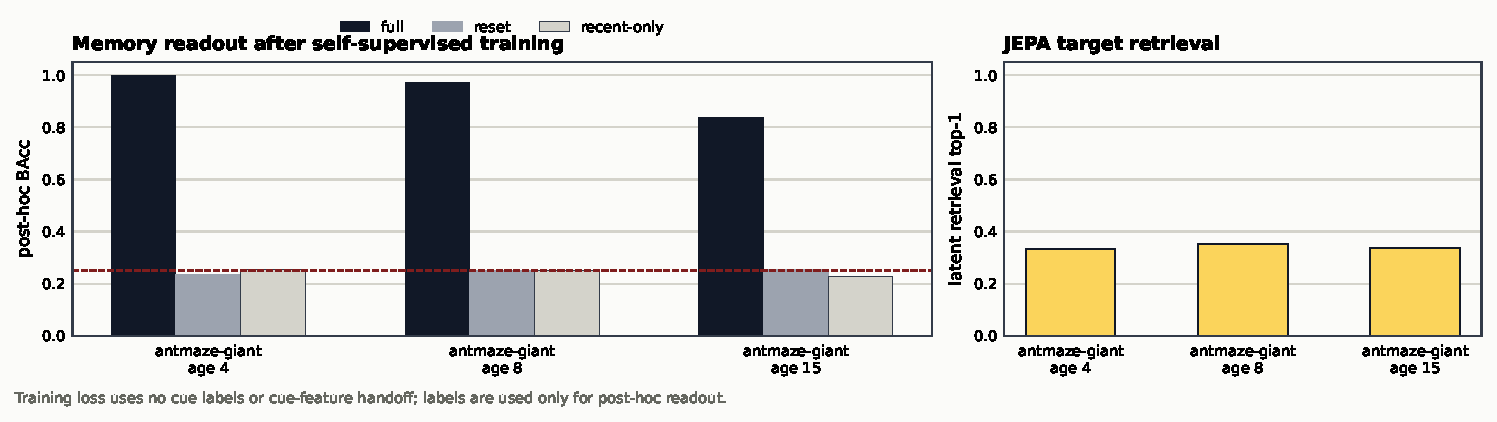
\includegraphics[width=\linewidth]{figures/fig_b_nonmanual_extra_antmaze_giant_navigate_v0.pdf}
\caption{Generated non-manual breadth plot for antmaze-giant-navigate-v0.}
\end{figure}

\begin{table}[!tbp]
\centering
\scriptsize
\setlength{\tabcolsep}{3.5pt}
\renewcommand{\arraystretch}{1.05}
\caption{Generated non-manual breadth table for antmaze-giant-navigate-v0.}
\begin{tabular}{lccccccl}
\toprule
Deck & Age & Seeds & Pass & Full & Reset & Recent & Status\\
\midrule
antmaze-giant-navigate-v0 & 4 & 3 & 3/3 & 1.000 & 0.235 & 0.254 & \textsc{pass}\\
antmaze-giant-navigate-v0 & 8 & 3 & 3/3 & 0.972 & 0.250 & 0.250 & \textsc{pass}\\
antmaze-giant-navigate-v0 & 15 & 3 & 3/3 & 0.839 & 0.255 & 0.229 & \textsc{pass}\\
\bottomrule
\end{tabular}
\end{table}

\paragraph{humanoidmaze-large-navigate-v0.}
This generated block reports 0/3 environment-age rows passing the
registered non-manual gate. Mixed rows are treated as stress-test limits or
confirmation targets, not as headline wins.

\begin{figure}[!tbp]
\centering
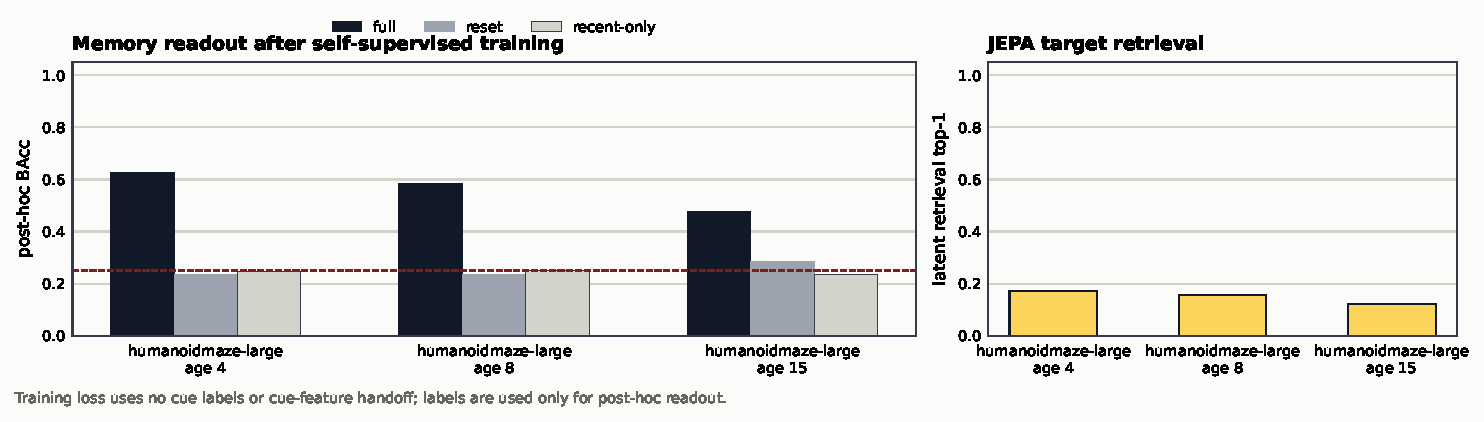
\includegraphics[width=\linewidth]{figures/fig_b_nonmanual_extra_humanoidmaze_large_navigate_v0.pdf}
\caption{Generated non-manual breadth plot for humanoidmaze-large-navigate-v0.}
\end{figure}

\begin{table}[!tbp]
\centering
\scriptsize
\setlength{\tabcolsep}{3.5pt}
\renewcommand{\arraystretch}{1.05}
\caption{Generated non-manual breadth table for humanoidmaze-large-navigate-v0.}
\begin{tabular}{lccccccl}
\toprule
Deck & Age & Seeds & Pass & Full & Reset & Recent & Status\\
\midrule
humanoidmaze-large-navigate-v0 & 4 & 3 & 1/3 & 0.626 & 0.234 & 0.247 & \textsc{mixed}\\
humanoidmaze-large-navigate-v0 & 8 & 3 & 0/3 & 0.585 & 0.236 & 0.250 & \textsc{mixed}\\
humanoidmaze-large-navigate-v0 & 15 & 3 & 0/3 & 0.476 & 0.285 & 0.236 & \textsc{mixed}\\
\bottomrule
\end{tabular}
\end{table}

